\documentclass[10pt]{article}
\usepackage{../local}


\newcommand{\classcode}{Physics 105}
\newcommand{\classname}{Analytic Mechanics}
\renewcommand{\maketitle}{%
\hrule height4pt
\large{Eric Du \hfill \classcode}
\newline
\large{HW 01} \Large{\hfill \classname \hfill} \large{\today}
\hrule height4pt \vskip .7em
\normalsize
}
\linespread{1.1}
\begin{document}
    \maketitle
    \section*{Problem 1}

    A mas $m$ is attached to a spring with spring constant $k$ and set oscillating in a dissipative medium. The mass' position $x(t)$ satisfies the differential equation

    \[ m \ddot x + b\dot x + kx = 0\] 

    where $b$ is the damping coefficient. Define the total energy as $E = T + V = \frac 12 m\dot x^2 + \frac 12 k x^2$. Calculate $\frac{dE}{dt}$ ad show it is equal to the rate at which work is done by friction.

    \begin{solution}
        If we take the time derivative of energy: 
        \[ \frac{dE}{dt} = m \dot x \ddot x + k x \dot x = \dot x(m \ddot x + kx) = -b\dot x^2\]

        Furthermore, we know that the work done by friction is $W = -bx$, so therefore: 

        \[ \frac{dW}{dt} = -b\dot x \frac{dx}{dt} = -b \dot x^2 = \frac{dE}{dt}\] 

        as desired. 
    \end{solution}
    \pagebreak

    \section*{Problem 2}

    A mass $m$ sits in the one-dimensional potential

    \[ V(r) = -\frac Ar + \frac{B}{r^2}\] 

    where $r > 0$, and $A$ and $B$ are positive constants. This kind of potential arises in studying gravitaitonal orbits, with the first term is due to gravitational potential, and the second is due to angular momentum conservation. 

    \begin{enumerate}[(a)]
        \item Sketch the potential for $r > 0$. Indicate on your graph the behavior of the potential for small and large $r$
        
        \begin{solution}
            Here's a plot below: 

            \begin{center}
                \begin{tikzpicture}[scale=0.5]
                    \draw[domain=1:10, samples=500, color=red] plot (\x, {-6/\x + 3/(\x^2)});
                    \draw[domain=0.34:1, samples=500, color=blue] plot (\x, {-6/\x + 3/(\x^2)});
                    \draw node at (7, 8) {$V = -\frac{A}{r} + \frac{B}{r^2}$};
                    \draw[very thick, -stealth] (0, 0) -- (11, 0) node[right] {$r$};
                    \draw[very thick, -stealth](0, -5) -- (0, 10) node[above]{$V(r)$};
                    \draw[color=red] (5.3, -1.4) node[below] {$V \approx -\frac{A}{r}$};  
                    \draw[color=blue] (0.36, 4) node[right] {$V \approx \frac{B}{r^2}$};
                    \draw[dashed]  (1, 0)node[above] {$r_0$} -- (1, -3) ;
                \end{tikzpicture}
            \end{center}

            It's not entirely true that the behavior for small and large $r$ switches exactly at the minimum, but I just had to choose a convenient point to show the different regimes. $r_0$ is also indicated on this graph to show the location of the minimum. 
        \end{solution}
        \item Your graph should indicate that there is a stable equilibrium. Find this equilibrium position $r_0$ and show that it is indeed stable. 
        
        \begin{solution}
            To solve for the equilibrium position, then we require that $V'(r) = 0$, so therefore: 

            \begin{align*}
                V'(r) &= \frac{A}{r^2} - \frac{2B}{r^3}\\
                \frac{A}{r^2} &= \frac{2B}{r^3}\\
                \therefore r_0 &= \frac{2B}{A}
            \end{align*}

            To show that it is indeed a stable equilibrium, we compute the second derivative: 

            \begin{align*}
                V''(r) &= \frac{-2A}{r^3} + \frac{6B}{r^4}\\
                V''(r_0) &= \frac{-2A}{\left(2B/A\right)^3} + \frac{6B}{(2B/A)^4}\\
                &= -\frac{A^4}{4B^3} + \frac{3A^4}{8B^3}\\
                &= \frac{A^4}{8B^3}
            \end{align*}

            And since $A$ and $B$ are positive constants, then $V''(r_0) > 0$, and so $V(r)$ is concave up at $r_0$, making the point stable.
        \end{solution}
        \item What is the period of small oscillations about this equilibrium $\omega$?
        
        \begin{solution}
            We know from discussion that we can taylor expand $V(r)$ in order to get an approximate solution. Specifically, we discussed that $V''(r_0) \equiv k$, from which we can find $\omega$. So therefore, 

            \[ V''(r_0) = k = \frac{A^4}{8B^3} \implies \omega = \sqrt{\frac{A^4}{8mB^3}}\]
        \end{solution}
        \item For a planet orbiting the sun, $A = GmM$ and $B = L^2/2m$, where $M$ is the mass of the sun. Show that $\omega$ is also the angular velocity of the planet about the sun. (\textit{This is remarkable - even if perturbed from a circular orbit (i.e. sitting at constant $r(t) = r_0$), planets will execute closed orbits since tehy oscillate once about their equilibrium radius once an orbit. Of course, even for significant deviations from equilibrium, their orbits are closed, since planets' trajectories are ellipses, as we will study later in this course.})
        
        \begin{solution}
            We know that $A = GMm$, and $B = L^2/2m = (mvr)^2/2m$. Pluggin these into $\omega$, we get (skipping a little bit of algebra):

            \begin{align*}
                \omega &= \frac{G^2M^2}{v^3r^3} = \frac{G^2M^2}{\omega^3r^6}\\
                \therefore \omega^4 &= \frac{G^2M^2}{r^6} \implies \omega^2 = \frac{GM}{r^3}
            \end{align*}

            We also know that from laws of circular orbits: 

            \begin{align*}
                m\omega^2r &= \frac{GMm}{r^2} \\
                \omega^2 &= \frac{GMm}{r^3}
            \end{align*}

            and since the equations are the same, we are done.
        \end{solution}
    \end{enumerate}

    \pagebreak

    \section*{Problem 3}

    Consider the following spring-mass setup. 
    
    \begin{center}
        \begin{tikzpicture}
            \draw (-3,0) -- (0,0);
            \draw[dashed] (0,0) -- (0,3) node[right] {$A$} node[midway, right] {$l$};
            \filldraw[black] (-2,0) circle (0.075cm);
            \node at (-2,-0.25) (m) {$m$};
            \draw (-2,0) -- (0,0) node[midway, below] {$x$};
            \draw [decoration={aspect=0.3, segment length=2.5mm, amplitude=1mm,coil},decorate] (0,3) -- (-2,0);
        \end{tikzpicture}
    \end{center}

    The mass $m$ is constrained to move along a horizontal line and is attached to a spring whose other end is fixed at $A$ at a distance $\ell$ from the horizontal line. The spring has a natural length of zero, and the force required to extend the spring to length $\ell$ is $F$. Find the frequency of small oscillations of the particle about its equilibrium position.

    \begin{solution}
        Let the angle between the horizontal line and the spring be $\theta$. We know then that the restoring force is $f = F \cos \theta$, but under small oscillations, $\cos \theta \approx 1$, so therefore we can just consider the spring to be stretched to length $\ell$ and so the restoring force is $F$. We also know from Hooke's law that $F = \ell k$, and so therefore $k = \frac{F}{\ell}$. Thus, 

        \[ \omega = \sqrt{\frac km} = \sqrt{\frac{F}{\ell m}}\] 
    \end{solution}

    \pagebreak

    \section*{Problem 4}
    During the spinning cycle in a washing machine, the clothes are forced into a centrifuge to squeeze the remaining water out of the machine. However, as the angular velocity of the machine increases, the centrifugal fixture (i.e. the spinning drum with the clothes inside) can go into resonance. This would cause the machine to break if the resonance is maintained, as the whole machine would shake apart. In modern washing machines, there are sensors and various electronics which prevent this from happening (or lasting too long). Describe why this resonance occurs by using an idealized physical model. You do not need to write down any equations, but a detailed description of the physics along with a model is necessary. (Hint: for an ordinary oscillating mass on a spring, resonance comes from an external force driving the mass at the oscillator's characteristic frequency. How might we model this system simliarly?)


    \begin{solution}
        Consider the washing machine system as effectively a mass $m$ on a hoop of mass $M$: 

        \begin{center}
            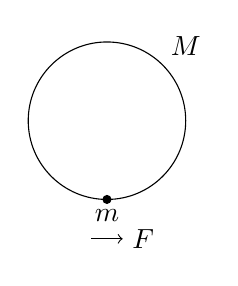
\begin{tikzpicture}
                \draw [radius=1cm] (0,0) circle;
                \filldraw (0, -1) circle (0.05) node[below] {$m$}; 
                \draw[->] (-0.2, -1.5) -- (0.2, -1.5) node[right] {$F$};
                \node[above] at (1, 0.7) {$M$};
            \end{tikzpicture}
        \end{center}

        Now suppose that a periodic force $F$ (the periodicity is required for resonance) pushes on the mass so that it goes around the hoop. If the frequency $\omega$ of the driving force is exactly at the angular velocity $\omega_0$ of the mass reaching the base of the hoop, then the mass will be accelerated around the hoop at a larger angular velocity. Since the mass is still constrained to move on the circle, the centrifugal force (or the centripetal force from an inertial frame) must be larger, and thus this causes greater forces to be exerted on our washing machine. If this continues, then eventually the centripetal force required to keep the mass constrained will be too large, and the washing machine falls apart (and then you now have wet clothes everywhere). 
    \end{solution}

    % \pagebreak

    \section*{Feedback}

    \begin{enumerate}[(a)]
        \item About how long did you spend on this homework?
        
        I spent about 3-4 hours on this homework (that includes typesetting this document), though I imagine the content to get harder so I think this number will end up going to about 6-7 hours later in the semester.


        \item Do you have any other feedback at this point in the course?
        
        My main issue right now is the fact that the slides go by way too fast. I feel like sometimes I simply don't have enough time to copy down the relevant information on the slides before the slides are already gone. This sentiment is also corroborated by my other friends who are in the class as well.

        Also, I personally don't \textit{love} physics lectures being presented on slides; I'd much prefer if it were taught using a blackboard, but at the moment the format is ok $-$ just the slides go by a bit too fast.


    \end{enumerate}

\end{document}